%
% A simple LaTeX template for Books
%  (c) Aleksander Morgado <aleksander@es.gnu.org>
%  Released into public domain
%

\documentclass[11pt]{book}
\usepackage[a4paper, top=3cm, bottom=3cm]{geometry}
\usepackage[latin1]{inputenc}
\usepackage{setspace}
\usepackage{graphicx}
\usepackage{fancyhdr}
\usepackage{tocloft}
\renewcommand{\familydefault}{\sfdefault}


\begin{document}


\pagestyle{empty}
%\pagenumbering{}
% Set book title
\title{\textbf{Need to discard this page}}
% Include Author name and Copyright holder name
\author{Whatever}



% 1st page for the Title
%-------------------------------------------------------------------------------
\maketitle


% 2nd page, thanks message
%-------------------------------------------------------------------------------


% General definitions for all Chapters
%-------------------------------------------------------------------------------

% Define Page style for all chapters
\pagestyle{fancy}
\fontsize{25pt}{20pt}\selectfont
% Delete the current section for header and footer
\fancyhf{}
% Set custom header
\lhead[]{\thepage}
\rhead[\thepage]{}

% Set arabic (1,2,3...) page numbering

% Set double spacing for the text
\doublespacing



% Not enumerated chapter
%-------------------------------------------------------------------------------
\chapter*{Acknowledgement}

This undertaking has received the whole-hearted support of many individuals. We are grateful to our department for providing us with this course communication and soft skills lab.We would also like to thank the department of English in training us in this course.Our heartfelt thanks goes to our respected English madam Athma Dharshana Pharee for the meticulous planning and guiding us in all possible ways in implementing this survey.We would also thank all those who imparted their value added time, effort in filling the questionnaires,and providing us with the required  data.
\\\\
The survey and the report prepared is an effort of our vibrant team. Firstly we  thank our entire team for their valuable contribution to make this report a talk among everyone.
We sincerely acknowledge the interest shown in our survey by our teachers, friends and other people who willingly shared their opinion on the privacy issues in social networking sites, they believe in. Their contribution has helped us in drawing a conclusion about the various threats faced by users of social networking sites.
% If the chapter ends in an odd page, you may want to skip having the page
%  number in the empty page
\newpage
\thispagestyle{empty}

\chapter*{Preface}

This  report  presents  findings about the various kinds of privacy issues and  threats faced by users of social networking sites. The main objective of the survey was to get information on levels of usage of social networking sites among different age groups of people over a specific period of time.A total of 75 people of various category such as college students,school students,teachers,engineers,householders were surveyed.
\\We have performed this survey in both micro and macro levels. At the micro-level, our survey begins with an individual, snowballing as social relationships are traced, or we started  with a small group of individuals in a particular social context. Rather than tracing interpersonal interactions, at macro-level analysis we  traced the outcomes of interactions, such as economic or other resource transfer interactions over a group of people.
\\The questionnaires covered a wide range of areas dealing in detail about all possible threats that would have been encountered by the users.We collected information on a wide range of  characteristics such as what type of information is mainly shared by users and  with whom. The information on the characteristics of the communities have been analyzed and presented in a separate report.
\\Numerous studies and research is being conducted nowadays on privacy issues in social networking sites.Various fields where they conduct study on social networking issues are :
\begin{itemize}
	\item \textbf{ORGANISATIONAL STUDIES:}\\
		Research studies of  formal or informal organizational relationships, organizational communication, economics, economic sociology, and other resource transfers. Social networks have also been used to examine how organizations interact with each other, characterizing the many informal connections that link executives together, as well as associations and connections between individual employees at different organizations. \\\\Intra-organizational networks have been found toaffect organizational commitment, organizational identification, interpersonal citizenship behaviour.
	\item \textbf{SOCIAL CAPITAL: }\\
		Social capital is a sociological concept which refers to the value of social relations and the role of cooperation and confidence to achieve positive outcomes. The term refers to the value one can get from their social ties. For example, newly arrived immigrants can make use of their social ties to established migrants to acquire jobs they may otherwise have trouble getting (e.g., because of lack of knowledge of language). \\\\Studies show that a positive relationship exists between social capital and the intensity of social network use.

	\item \textbf{HUMAN ECOLOGY: }\\
		Human ecology is an interdisciplinary and transdisciplinary study of the relationship between humans and their natural, social, and built environments. 
		\\\\In criminology and urban sociology, much attention has been paid to the social networks among criminal actors.
		\\\\It is expected that this report will be a useful source of information to policy makers, academicians and other stakeholders. It will also facilitate planning within the government and the business community and will stimulate further research and analysis.
\end{itemize}

% If the chapter ends in an odd page, you may want to skip having the page
%  number in the empty page
\newpage
\thispagestyle{empty}


% First enumerated chapter
%-------------------------------------------------------------------------------
\tableofcontents
\pagenumbering{arabic}
\chapter{Introduction}
This  survey  report  presents   latest  information  from  the  general  lifestyle  survey . The  topic  for the survey was social networking  privacy issues  . 
Survey  was  mainly conducted  for people  of  all  ages  from  all  walks  of  life.  
The  survey  was  aimed  at finding the amount of trust people have on various sites and amount of information people share. 
The survey was conducted by circulating a questionnaire among people and  representing their answers in form of pie diagrams and bar graphs. 
Generally people supply all kinds of information on the sites including their personal information , photographs , contact details and so on. 
\\\\They also consider that these details provided by them are secure and people other than their friends do not know these. 
But on the contrary the site developer's team maintains a database of the kind of information shared by people along with their details and may use them whenever needed. 
This is done with the consent of the particular person but it often goes unnoticed by the people because they do not read the license agreement of the company fully instead they agree to the terms and conditions of the company. 
\\\\Our survey comprises of the following sections - title page , executive summary of the survey , content page,  our methodology using which we conducted our survey , the results and findings of our survey , the conclusions which were drawn from the survey , our recommendations and suggestions  ,  appendices , bibliography and acknowledgements.  
\\\\Our survey questionnaire exposed people to various kinds of information which they might generally not come across in their day to day basis while using these sites. Our survey mainly targeted fragile security issues which are a cause of concern for the people. The survey showed that almost 70\% of the people were unaware of the security measures that could be taken to maintain their privacy. We mainly wanted to make people know that their ids and passwords are not actually meant for their privacy. Though they keep them secure to certain extent they do not prevent the companies from using this code and accessing the users private information. \\\\Instead the TOR ( the onion router) can be used so that the identity of the user remains hidden from the company's perspective and  hence the user can stay more private from the service provider. \\\\Even sites like diaspora can be used by people in which their information remains secure and safe and no other person can access it without the consent of the particular user. These options can be implemented because the results from our survey show that people share more personal information like their photos , relationship status , contact details etc on these sites which might cause them trouble if not handled properly. \\\\Moreover we also have supporting pie charts and bar graphs to stress on the same. These show that people are unaware of various security issues and are still using these sites by fully trusting them. \\\\Our recommendations gives an insight into various other options which can be used for the benefit of the society . \\\\Our survey was mainly conducted for the purpose of benefitting the society by throwing light into the issues they are unaware of and also providing them with solutions for the same. \\\\We also have an appendix to  provide insight into various terminologies used in our survey. \\\\Also we have an bibliography and acknowledgement  that coincides with the content provided in our survey. \\\\On the whole our survey completely addresses all issues concerned with the topic and also provides solutions and recommendations which can be followed by the people to keep them secure at all times.
\chapter{Methodology}
We mainly concentrated on two methodologies - Questionnaires and Discussions
\begin{enumerate}
	\item Questionaire \\We created fifty copies of our questionaires. I will be attaching the set of questions asked. 
	\item Discussions \\After having the group discussions in our class, a new sense of confidence grew within us. 
		We conducted several discussions among ourselves on what kind of conclusions would arise from this survey report. 
		And how each result could be used to draw some kind of a conclusion. 
	\item Interviews \\We interviewed a few people and included the results of the same in our analysis as well. 
		All the people we interviewed were mostly people working currently. Notably : 
		\begin{itemize}
			\item Asst. Prof Bama Ma'am, Dept of IST, CEG
			\item Sibi Chakravarthy - IAS Aspirant
			\item Prasanth Radhakrishnan - Sub Editor Hindu
			\item Welkin - Entreprenuer
		\end{itemize}
\end {enumerate}
\chapter{Question 1}

\begin{figure}[ht!]
	\centering
	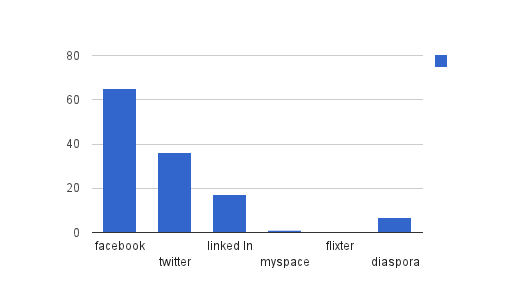
\includegraphics[width=150mm]{1.png}
	\caption{Richard Stallman and Julien Assange}
	\label{overflow}
\end{figure}
\\\textbf{}

\newpage
\chapter{Conclusions}
We must opt out of global data surveillance programs like PRISM, XKeyscore and Tempora. Stop governments from spying on you by encrypting our communications and ending our reliance on proprietary services.
Here is a timeline of the companies that joined the Prism Project.
\begin{figure}[ht!]
	\centering
	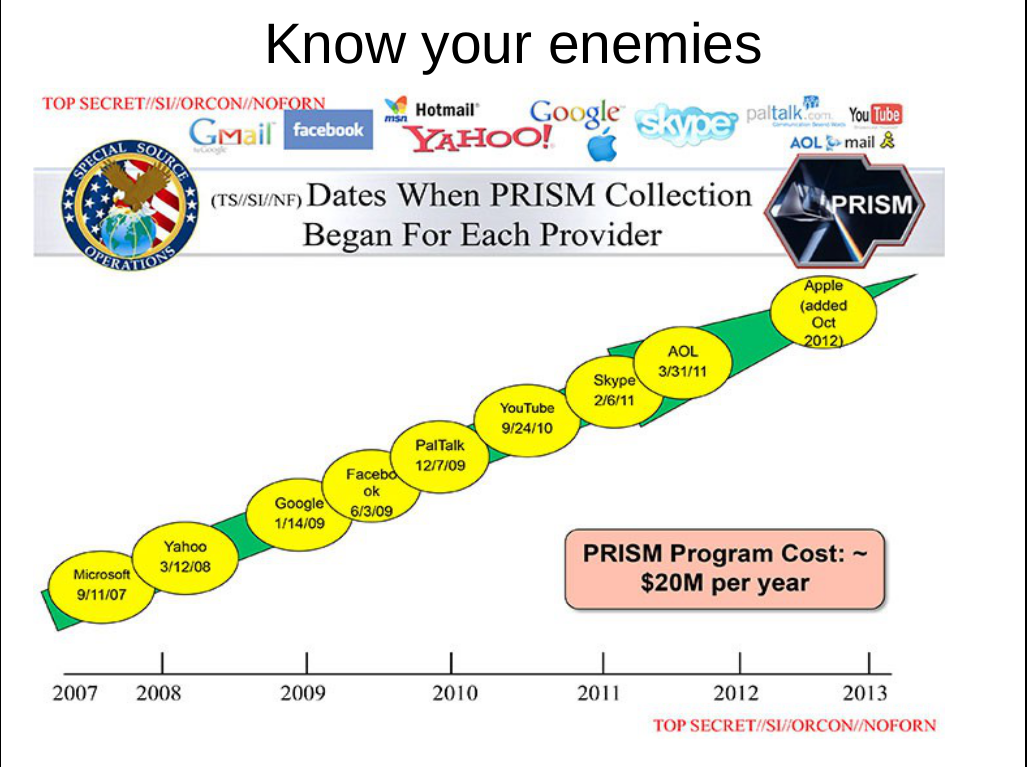
\includegraphics[width=150mm]{prism1.png}
	\caption{Prism Project Timeline}
	\label{overflow}
\end{figure}
\newpage

\begin{figure}[ht!]
	\centering
	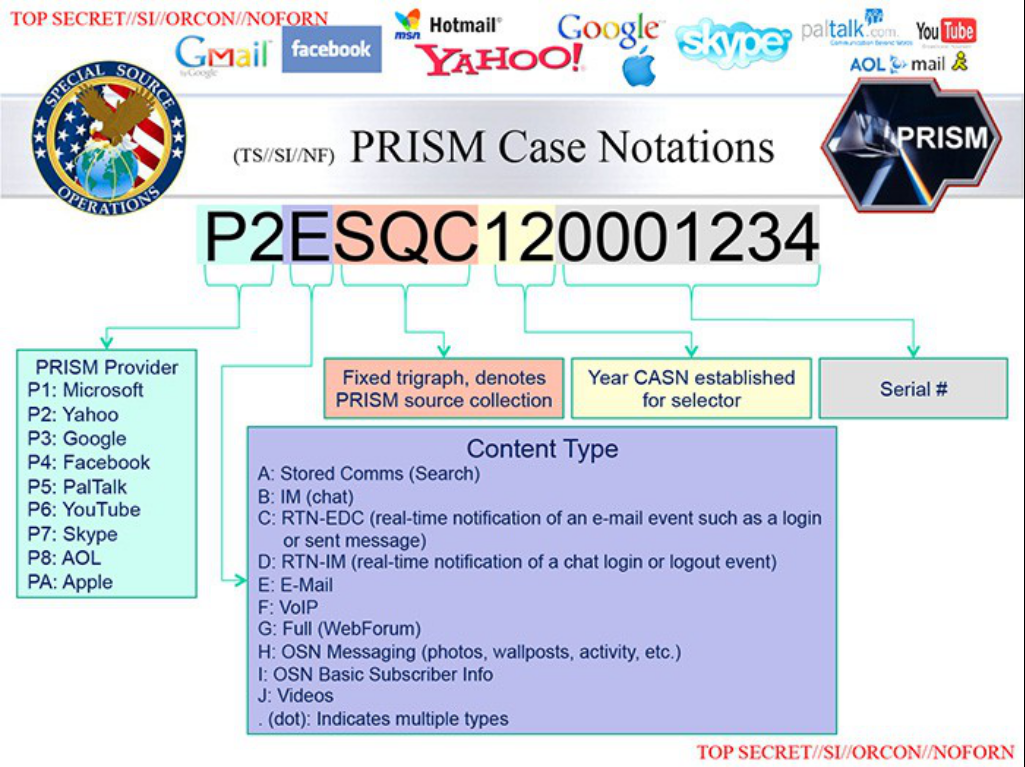
\includegraphics[width=150mm]{prism2.png}
	\caption{Notations used in the Prism Project}
	\label{overflow}
\end{figure}
\newpage
Here is a list of a few greats who took steps much bigger than what we are taking. 
They took it up as a challenge at fought for one major cause\ldots
\\\\\emph{Knowledge is free}\\\\
\begin{figure}[ht!]
	\centering
	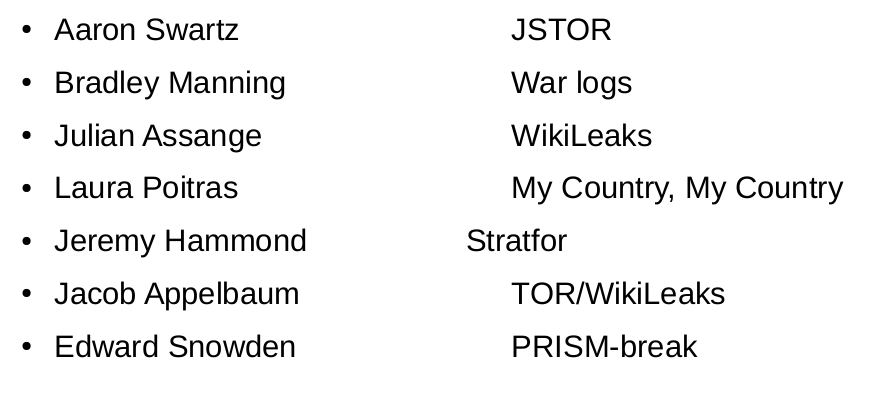
\includegraphics[width=150mm]{prism3.png}
	\label{overflow}
\end{figure}
\newpage
Here is what was their fate. \\\\ It feels really sad to see their current state. Whatever they have done, would help the world become a better place in the years to come. 
\begin{figure}[ht!]
	\centering
	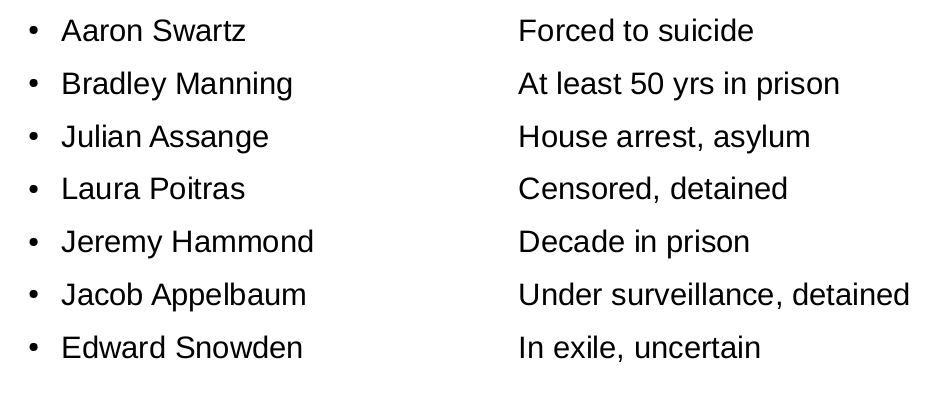
\includegraphics[width=150mm]{prism4.png}
	\label{overflow}
\end{figure}
\\\\We take pride in the fact that we have a role in making the internet a safer place as well.
\\ We are telling people that they shouldn't blindly trust some random third person they have never met. Trusting someone you know is a much better option. 
\newpage
These two public figures are shown to Back Edward Snowden for his great contribution. 
\\If not for his contributions, the world would not have known about these ``Cyber Atrocities'' committed by the NSA. 
\begin{figure}[ht!]
	\centering
	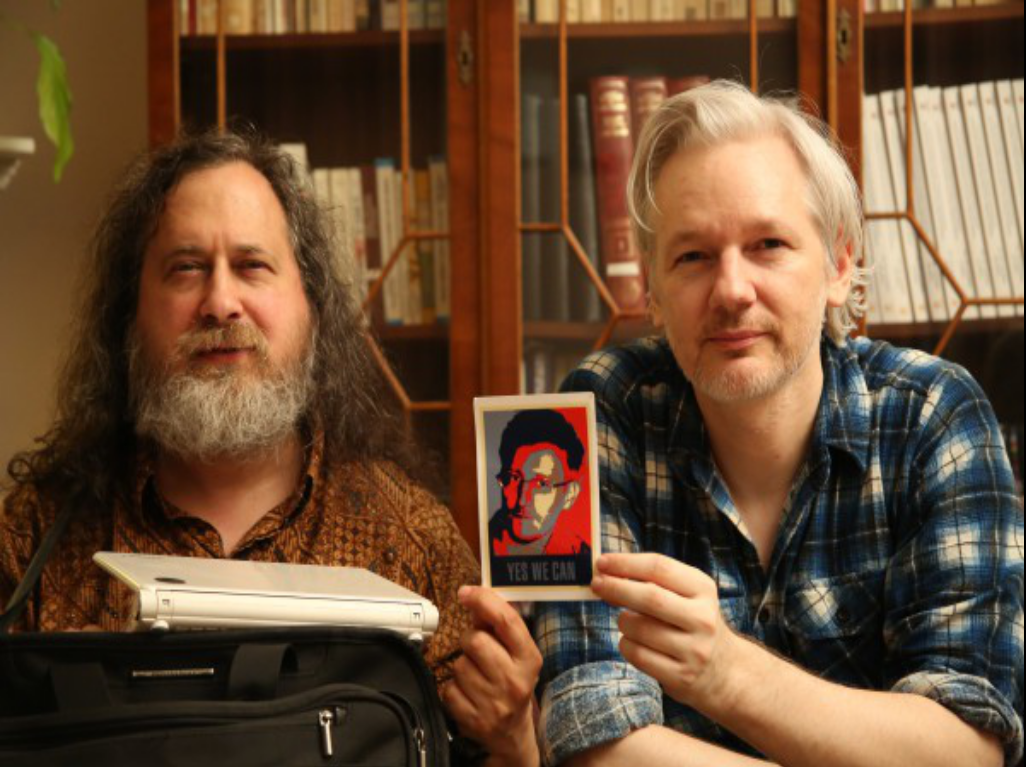
\includegraphics[width=150mm]{prism5.png}
	\caption{Richard Stallman and Julien Assange}
	\label{overflow}
\end{figure}
\newpage

% Last pages for ToC
%-------------------------------------------------------------------------------
\newpage
\chapter{Recommendations}
A recommendation is anything that serves to recommend a person or thing, or induce acceptance or favor. 
\\\emph{Source: Dictionary.reference.com}

\\So what big thing did we find that we are going to recommend changes? 
\begin{itemize}
	\item The first recommendation would be, many are still not aware of the Social Networking Problems.
		We need to hold proper rallies, campaigns to help people understand the problem they are in.
	\item People rely on one solution too much. It is a bad business strategy and kills competition. Most 
		citizens are oblivious to this fact. 
	\item Setting up a server in our campus. For Diaspora, Gitlab would do a lot of good.
	\item \emph{Knowledge must be free, always} . (Free as in freedom) . There should be no digital restrictions on knowledge. 
		Books must not have digital laws binding them, saying that I should not give it to anyone. 

\end{itemize}
\newpage
\chapter{Bibliography}
\begin{enumerate}
	\item duckduckgo.com
	\item https://en.wikipedia.org/wiki/Diaspora
	\item Check out our live form online at https://docs.google.com/forms/d/1NX11AXxvFVWBA0Yy2CiHZtJSdD3N-w4t9Sw4mmpIf8g/viewform
	\item https://www.quora.com/search?q=julian+assange
	\item https://prism-break.org/
	\item https://fsf.org/campaigns/
	\item http://fsftn.org/content/software-freedom-week
	\item http://fsmk.org/?q=sunday-school
	\item https://stackoverflow.com
	\item https://uncyclopedia.com
\end{enumerate}
\newpage
\chapter{Appendix A - Glossary}
FSF : Free software foundation\\
FSFTN : Free software Foundation Tamil Nadu\\
Diaspora : Its a distributed Social network\\
Duckduckgo : A search engine, supposed to be better than google in terms of encryption\\
FSMK : Free software movement Karnataka\\
TOR: Its a network which supports privacy by policy, and not by trust.\\

\newpage
\chapter{Appendix B- Survey Questions}
\newpage
\chapter{Appendix C -Survey result sheet}
\newpage
% Include dots between chapter name and page number
\renewcommand{\cftchapdotsep}{\cftdotsep}
%Finally, include the ToC



\end{document}
